\documentclass{article}

\usepackage{hyperref}
\usepackage{amsmath}
\usepackage{graphicx}
\usepackage{subcaption}
\usepackage{epstopdf}
\usepackage{color}

\usepackage{times}
\usepackage{bm}

% Page layout
\hoffset -0in
\voffset -1in
\oddsidemargin 0in
\textheight 9.3in
\textwidth 6.3in

\setlength{\parindent}{0pt}
%\setlength{\intextsep}{10pt}
%\pagestyle{empty}

\graphicspath{{figures/}}

\begin{document}
	\section*{COMPUTATIONAL METHODS IN MECHANICS: Assignment 5}
	Vesa-Ville Hurskainen, 21 Feb 2018\\
	\href{https://github.com/VesaVilleHurskainen/cmim2018}{GitHub repository}

	\section*{Introduction}
	This is a report of the fifth assignment of the course \textit{Computational Methods in Mechanics}. The assignment consists of five tasks, which are as follows:
	\begin{enumerate}
		\setlength\itemsep{0pt}
		\item To implement backward Euler method using Newton-Raphson.
		\item To derive equations of motion for a given mass-rod system.
		\item To derive Jacobian matrix for the system using symbolic computations.
		\item To solve the system using backward Euler method and the previously derived Jacobian.
		\item To solve the system using ode15s and compare the results. Then investigate if ode15s is faster or more accurate with a provided Jacobian and discuss how the solver can compute a solution even without one.
	\end{enumerate}

	\section*{Methods}
	The system's equations of motion were derived using the Lagrangian method. Supposing that the rod is attached to the midpoint of the mass, the system's kinetic and potential energy functions and the resulting Lagrangian are as follows:
	\begin{equation}
		\begin{aligned}
		T &= \frac{1}{2} m \dot{x}^2 + \frac{1}{2} \int_{0}^{l} m_l \left[ \left( \frac{d}{dt} (x + y \sin \theta) \right)^2 + \left( \frac{d}{dt} (y \cos \theta) \right)^2 \right] dy \\
		U &= \frac{1}{2} k x^2 + k (x + l \sin \theta)^2 \\
		L &= T - U
		\end{aligned}
	\end{equation}
	where $m_l = 2 m / l$ is rod mass per unit length and $y$ is rod lengthwise coordinate, starting from the joint. Defining the generalized coordinates $\bm{q} = \begin{bmatrix} x & \theta \end{bmatrix}^\text{T}$, we get the Lagrange equation:
	\begin{equation}
		\frac{d}{dt}\left(\frac{\partial L}{\partial \dot{\bm{q}}}\right) - \frac{\partial L}{\partial \bm{q}} = \frac{\partial D}{\partial \dot{\bm{q}}}
	\end{equation}
	where the nonconservative forces caused by dampers are accounted for using the Rayleigh dissipation function:
	\begin{equation}
	D = - \frac{1}{2} c \dot{x}^2 - \frac{1}{2} c \left(\frac{d}{dt} (x + l \sin \theta) \right)^2
	\end{equation}	
	The accelerations of the system can be solved from the Lagrange equation via simple algebra, resulting in a system of two second order ODEs:	
	\begin{equation}
		\begin{aligned}
		\begin{bmatrix}
		\ddot{x} \\ \ddot{\theta}
		\end{bmatrix} =
		~&\mathbf{M}^{-1}
		\begin{bmatrix}
		- 3 k x - 4 c \dot{x} + l m \dot{\theta}^2 \sin \theta - 2 l c \dot{\theta} \cos \theta  - 2  l k \sin \theta\\
		- 2 l k \cos \theta (x + l \sin \theta) - 2 l c \cos \theta (\dot{x} + l \dot{\theta} \cos \theta) + l m \dot{\theta} \dot{x} \sin \theta
		\end{bmatrix}\\
		& \mathbf{M} =
		\begin{bmatrix}
		3 m & l m \cos \theta \\
		l m \cos \theta & 2 l^2 m / 3
		\end{bmatrix}
		\end{aligned}
	\end{equation}
	which is then further reduced to a system of four first order ODEs for computational purposes. The system's equations of motion were derived symbolically using script \texttt{system\_equations.m} and then solved using the script \texttt{assignment5.m}, which uses the backward Euler implementation of function \texttt{bwdEuler.m}. This, in turn, uses the function \texttt{newtonRaphson.m} for solving the nonlinear equations. The system's Jacobian matrix was derived symbolically in the script, using the above-presented equations of motion.
	
	\clearpage
	\section*{Results}
	The system was simulated using the parameters $m = 1$ kg, $c = 0.1$, $k = 100$ N/m, $l = 1$ m. An initial excitation was given by displacing the mass $0.1$ m. The simulation parameters were $\Delta t = 0.001$ s, $t = 0 \dots 5$ s. A comparison between the system's responses when computed using the backward Euler method and the MATLAB solver ode15s are presented in Figure~\ref{fig:response}. Another comparison between the responses computed with ode15s with and without provided Jacobian is presented in Figure~\ref{fig:jacobian}.\\
	
	\begin{figure}[h!]
		\centering
		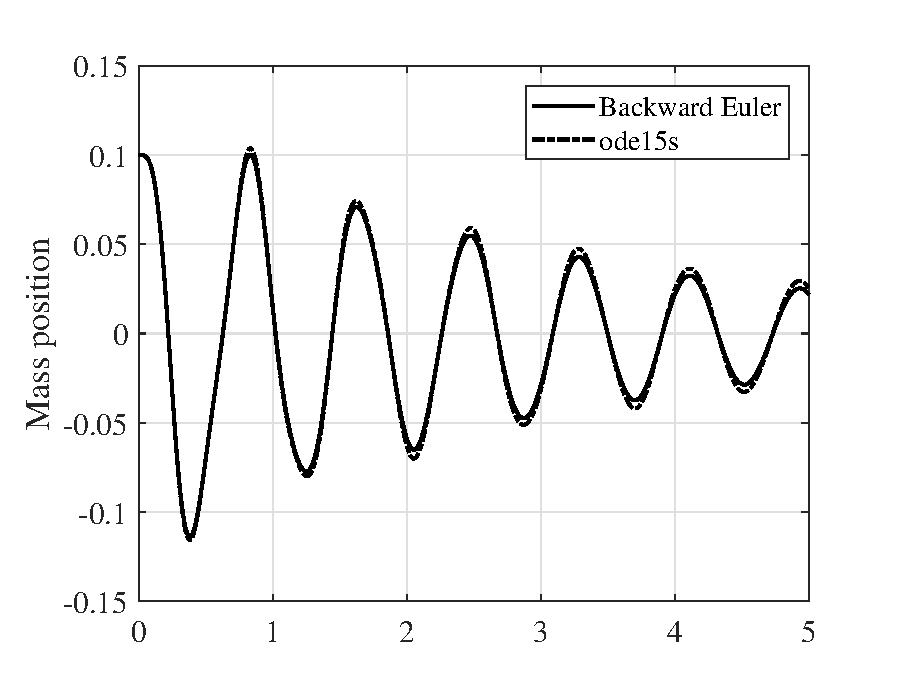
\includegraphics[width=0.45\textwidth]{response.eps}
		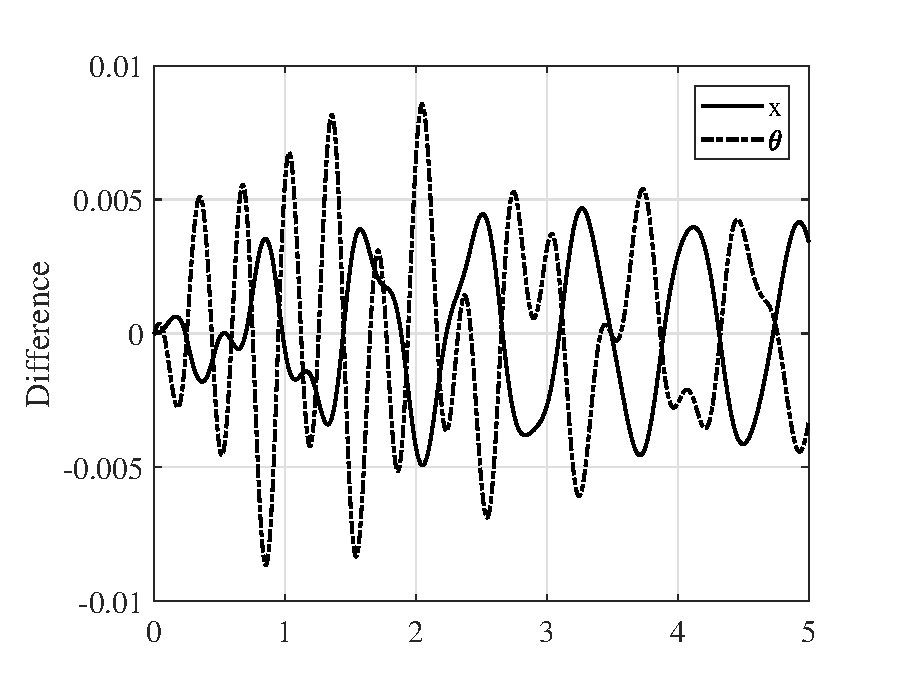
\includegraphics[width=0.45\textwidth]{diff_euler.eps}
		\caption{System response, comparison between backward Euler and ode15s with provided Jacobian.\label{fig:response}}
	\end{figure}

	\begin{figure}[h!]
		\centering
		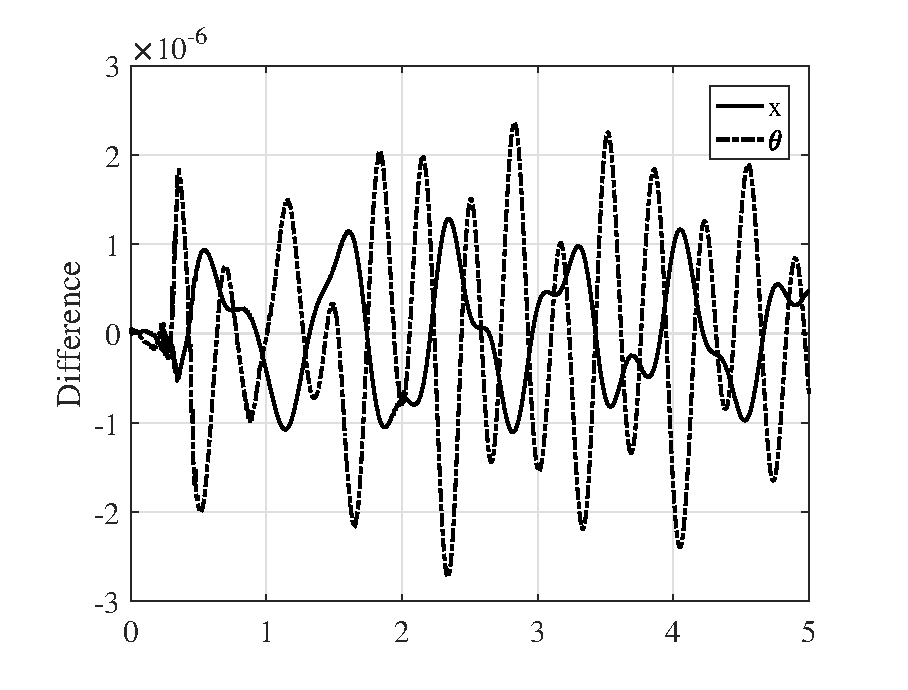
\includegraphics[width=0.45\textwidth]{diff_jac.eps}
		\caption{System response, difference between ode15s with and without Jacobian.\label{fig:jacobian}}
	\end{figure}

	Investigating the solver stats, the main difference between the computations with and without provided Jacobian was the number of function evaluations: 453 evaluations without Jacobian and 445 evaluations with Jacobian.
	
	\section*{Analysis}
	The results show relative agreement between backward Euler and ode15s, with maximum position error at roughly 5e-3 and angle error at 8e-3. However, this difference is strongly dependent on the time step; choosing a smaller time step shrinks the difference.\\
	
	The difference between ode15s computations with and without Jacobian were very small in the investigated case, as the scale of Figure~\ref{fig:jacobian} shows. A Jacobian can be computed from the system function via numerical differentiation (e.g.~finite difference method), which is why it is not strictly necessary to provide a Jacobian for many solvers.
\end{document}